\documentclass[../../../../main.tex]{subfiles}

\begin{document}

\subsection*{第1問}

[解] $P, Q$ が2辺 $CA, AB$ 上にある時, $P$ が $CA$, $Q$ が $AB$ 上にあるとして良い。
$|PA|=x, |QA|=y \quad (0 \le x \le 36, 0 \le y \le 25 \quad \cdots \text{①})$ とする。題意から
\[
xy = \frac{1}{2} \cdot 25 \cdot 36 = 450 \quad \cdots \text{②}
\]
$\triangle APQ$ で余弦定理から,
\[
\begin{aligned}
|PQ|^2 &= |AP|^2 + |AQ|^2 - 2 AP \cdot AQ \cos \angle PAQ \\
&= x^2 + y^2 - 900 \cos \angle PAQ
\end{aligned}
\]
$x^2, y^2 > 0$ から, AM-GM 及び ② から,
\[
|PQ|^2 \ge 900 (1 - \cos \angle PAQ) \quad \cdots \text{③}
\]
等号成立は $x=y=15\sqrt{2}$ の時成立する。ここで $\triangle ABC$ について余弦定理から,
\[
\cos \angle CAB = \frac{36^2 + 25^2 - 32^2}{2 \cdot 36 \cdot 25} = \frac{897}{2 \cdot 900}
\]
から, ③より,
\[
|PQ|^2 \ge \frac{903}{2} \quad \cdots \text{④}
\]
以下同様にして,
\begin{itemize}
  \item $P, Q$ が2辺 $AB, BC$ 上にある時
  \[
  |PQ|^2 \ge \frac{1247}{2} \quad (\text{等号成立は } |PB|=|QB|=20) \quad \cdots \text{⑤}
  \]
  \item $P, Q$ が2辺 $BC, CA$ 上にある時
  \[
  |PQ|^2 \ge \frac{609}{2} \quad (\text{等号成立は } |PC|=|QC|=24) \quad \cdots \text{⑥}
  \]
\end{itemize}
④, ⑤, ⑥から, もとめるのは,
\[
\text{2辺 } BC, CA \text{上の, } C \text{からの距離が } 24 \text{である2点.}
\]

\subsection*{第2問}

[解] $k, m \ge 1$ と仮定すると, 与式に $x=-1$ を代入して,
\[
0 - 1 = 0
\]
となり不適。よって, $k, m$ のうち少なくとも1つは $0$ である。 \quad \cdots \text{①}

さらに $x=1$ を代入して,
\[
2^k - 1 = 2^m \quad \cdots \text{②}
\]
$k=0$ とすると, $2^m = 0$ となり不適。したがって, ①とあわせて $m=0$ で, この時 $k=1$ である。与式に代入して
\[
\frac{x+1}{x^l} - 1 = \frac{1}{x^n} \quad \cdots \text{③}
\]
$l > n$ と仮定する。両辺に $x^l$ をかけて,
\[
x + 1 - x^l = x^{l-n}
\]
$n=0$ の時 ③で $x+1 = 2x^l$ となり不適だから, $n \ge 1$ であることとあわせて, 最高次を比較して $l=1$ が必要。しかしこの時, $0 < n < 1$, $n \in \mathbb{Z}$ となり矛盾。

同様に $l < n$ の時も矛盾するから, $l=n$ が必要である。この時, $l=n=1$ となる。(係数比較)

逆に $(k,m,n,l) = (1,0,1,1)$ の時, 与式は恒等式で、十分。

以上から
\[
(k, m, n, l) = (1,0,1,1)
\]

\subsection*{第3問}

[解] $x=t \ (0 < t < 4)$ で2つの図形が接するとする。この時, $y$ を消去した
\[
-ax^2 + bx = 4 - 2x
\]
\[
\therefore ax^2 - (b+1)x + 4 = 0 \quad \cdots \text{①}
\]
が $x=t$ を重解に持つ ($\because a \neq 0$)。判別式 $D$ として
\[
D = (b+1)^2 - 16a = 0 \quad \cdots \text{②}
\]
で, このもとで, 解は $x = \frac{b+1}{2a}$ だから, $t$ の値をいれて
\[
0 < \frac{b+1}{2a} < 4 \quad \cdots \text{③}
\]
となり, $a>0$ に注意して, 放物線の概形は右図で, 題意の面積 $S$ として
\[
S = \int_0^{b/a} (-ax^2+bx) \, dx = \frac{a}{6} \left(\frac{b}{a}\right)^3 = \frac{1}{6} \frac{b^3}{a^2} \quad \cdots \text{④}
\]
さて, ②から $a = \frac{(b+1)^2}{16}$ だから, ③④に代入して
\[
\begin{cases}
0 < \frac{16(b+1)}{(b+1)^2} < 4 \\[2mm]
S = \frac{16^2}{6} \frac{b^3}{(b+1)^4}
\end{cases}
\iff
\begin{cases}
1 < b \\[2mm]
S = \frac{8 \cdot 16}{3} \frac{b^3}{(b+1)^4} \quad \cdots \text{⑤}
\end{cases}
\]
ここで, $p = b+1$ とすると, ⑤から, $2 < p$ で,
\[
S = \frac{8 \cdot 16}{3} \frac{(p-1)^3}{p^4} = \frac{8 \cdot 16}{3} \left( \frac{1}{p} - \frac{3}{p^2} + \frac{3}{p^3} - \frac{1}{p^4} \right)
\]
$q = \frac{1}{p}$ として, $(0 < q < \frac{1}{2})$
\[
\begin{aligned}
\frac{dS}{dq} &= \frac{16 \cdot 8}{3} (1 - 6q + 9q^2 - 4q^3) \\
&= \frac{8 \cdot 16}{3} \left( q - \frac{1}{4} \right) (-4) (q - 1)^2
\end{aligned}
\]
だから, 下表をうる。

\begin{center}
\begin{tabular}{c|c|c|c|c|c}
$q$ & $0$ & $\dots$ & $1/4$ & $\dots$ & $1/2$ \\ \hline
$S'$ & & $+$ & $0$ & $-$ & \\ \hline
$S$ & & $\nearrow$ & & $\searrow$ &
\end{tabular}
\end{center}

したがって, $q = \frac{1}{4}$, つまり $(a, b) = (1, 3)$ の時 (⑤を満たす) $\max S = \frac{9}{2}$ をとる。

\begin{center}
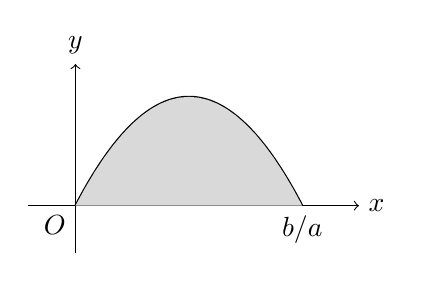
\begin{tikzpicture}[scale=1.2]
  \draw[->] (-0.5,0) -- (3.0,0) node[right] {$x$};
  \draw[->] (0,-0.5) -- (0,1.5) node[above] {$y$};
  \node[below left] at (0,0) {$O$};
  
  \draw[domain=0:2.4,samples=100,smooth,thick] plot (\x, {-0.8*\x*\x + 1.92*\x});
  \fill[gray!30] (0,0) -- plot[domain=0:2.4] (\x, {-0.8*\x*\x + 1.92*\x}) -- cycle;
  
  \node[below] at (2.4,0) {$b/a$};
\end{tikzpicture}
\end{center}

\subsection*{第4問}

[解] $a_1 = \sqrt{2} = 2 \sin \theta_1 \quad \therefore \theta_1 = \frac{\pi}{4} \quad \cdots \text{①}$ である。漸化式から
\[
\begin{aligned}
2 \sin \theta_{n+1} &= \sqrt{2 (1 + \sin \theta_n)} \\
&= \sqrt{2 \left( 1 + \cos \left(\frac{\pi}{2} - \theta_n\right) \right)} \\
&= \sqrt{4 \cos^2 \left( \frac{\pi}{4} - \frac{\theta_n}{2} \right)} \\
&= 2 \cos \left( \frac{\pi}{4} - \frac{\theta_n}{2} \right) \quad (\because 0 < \theta_n < \pi/2) \\
&= 2 \sin \left( \frac{\pi}{4} + \frac{\theta_n}{2} \right)
\end{aligned}
\]
だから, $0 < \theta_{n+1}, \frac{\pi}{4} + \frac{1}{2}\theta_n < \frac{\pi}{2}$ より,
\[
\theta_{n+1} = \frac{1}{2}\theta_n + \frac{\pi}{4}
\]
\[
\theta_{n+1} - \frac{\pi}{2} = \frac{1}{2} \left( \theta_n - \frac{\pi}{2} \right)
\]
①とあわせてくり返し用いて,
\[
\theta_n = \frac{\pi}{2} - \frac{\pi}{4} \left(\frac{1}{2}\right)^{n-1}
\]
であり,
\[
\theta_n \xrightarrow{n \to \infty} \frac{\pi}{2}
\]
となる。

\subsection*{第5問}

[解] (1) $r(n) = \frac{a}{2^n}$ とおく。 $O_n$ を原点とし, $\vec{O_n O_{n+1}}$ を $x$ 軸とする下図のような平面をとる。この平面での $S_n, S_{n+1}$ の断面は
\[
C_n : x^2 + y^2 = r(n)^2
\]
\[
C_{n+1} : (x - r(n))^2 + y^2 = r(n+1)^2
\]
であり, これらの交点の $x$ 座標は,
\[
x = \frac{-r(n+1)^2 + 2r(n)^2}{2r(n)} = \frac{7a}{2^{n+3}}
\]
である。ここで, $x, y$ 軸へ $\frac{2^n}{a}$ 倍した座標で考えれば, もとめる体積 $V_n$ は
\[
\begin{aligned}
\left( \frac{2^n}{a} \right)^3 V_n &= \pi \int_{\frac{7}{8}}^{\frac{1}{2}} \left\{ \frac{1}{4} - (x-1)^2 \right\} dx + \pi \int_{\frac{7}{8}}^1 (1 - x^2) dx \\
&= \pi \int_{\frac{1}{8}}^{\frac{1}{2}} \left( \frac{1}{4} - x^2 \right) dx + \pi \int_{\frac{7}{8}}^1 (1 - x^2) dx \quad \cdots \text{①}
\end{aligned}
\]
各項計算して,
\begin{itemize}
  \item $\displaystyle \int_{\frac{1}{8}}^{\frac{1}{2}} \left(\frac{1}{4} - x^2\right) dx = \left[ \frac{1}{4} x - \frac{1}{3} x^3 \right]_{\frac{1}{8}}^{\frac{1}{2}} = \frac{1}{4} \left( \frac{1}{2} - \frac{1}{8} \right) - \frac{1}{3} \left( \frac{1}{8} - \frac{1}{8^3} \right) = \frac{27}{8 \cdot 64}$
  \item $\displaystyle \int_{\frac{7}{8}}^1 (1 - x^2) dx = \left[ x - \frac{1}{3} x^3 \right]_{\frac{7}{8}}^1 = \frac{2}{3} - \left( \frac{7}{8} - \frac{1}{3} \left( \frac{7}{8} \right)^3 \right) = \frac{23}{3 \cdot 8^3}$
\end{itemize}
だから, ①より
\[
V_n = \pi \left(\frac{a}{2^n}\right)^3 \left\{ \frac{27}{8^3} + \frac{23}{3 \cdot 8^3} \right\} = \pi \left(\frac{a}{2^{n+3}}\right)^3 \cdot \frac{104}{3}
\]

(2)
\[
V_m = \frac{104 a^3 \pi}{3} \sum_{n=1}^m \left(\frac{1}{2^{n+3}}\right)^3 = \frac{104 a^3 \pi}{3} \left(\frac{1}{2^4}\right)^3 \frac{1 - (1/2)^{3m}}{1 - (1/2)^3} \xrightarrow{m \to \infty} \frac{13}{1344} a^3 \pi
\]

[注]
$V_n$ の求値に球帽公式を用いると,
\begin{itemize}
  \item $\displaystyle \int_{\frac{1}{8}}^{\frac{1}{2}} \left(\frac{1}{4} - x^2\right) dx = \frac{3/8}{2 \cdot 1/2} \cdot \frac{4}{3} \pi \left(\frac{1}{2}\right)^3 - \frac{1}{3} \left(\frac{\sqrt{15}}{8}\right)^2 \cdot \pi \cdot \frac{1}{8} = \frac{27 \pi}{8^3}$
  \item $\displaystyle \int_{\frac{7}{8}}^1 (1 - x^2) dx = \frac{1/8}{2 \cdot 1} \cdot \frac{4}{3} \pi - \frac{1}{3} \left(\frac{\sqrt{15}}{8}\right)^2 \cdot \pi \cdot \frac{7}{8} = \frac{23 \pi}{3 \cdot 8^3}$
\end{itemize}
と計算出来る。

\begin{center}
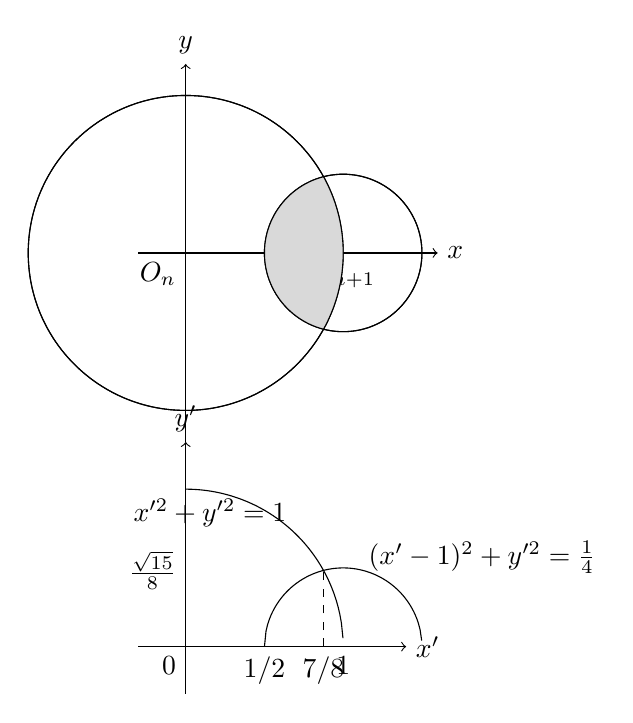
\begin{tikzpicture}[scale=2.0]
  \draw[->] (-0.3,0) -- (1.6,0) node[right] {$x$};
  \draw[->] (0,-1.2) -- (0,1.2) node[above] {$y$};
  \node[below left] at (0,0) {$O_n$};
  
  \draw (0,0) circle (1);
  \draw (1,0) circle (0.5);
  \node[below] at (1,0) {$O_{n+1}$};
  \node[below right] at (0.5,0) {$\frac{a}{2^n}$};
  
  \begin{scope}
    \clip (0,0) circle (1);
    \clip (1,0) circle (0.5);
    \fill[gray!30] (-1,-1) rectangle (2,1);
  \end{scope}
  \draw (0,0) circle (1);
  \draw (1,0) circle (0.5);
  
  \begin{scope}[shift={(0,-2.5)}]
    \draw[->] (-0.3,0) -- (1.4,0) node[right] {$x'$};
    \draw[->] (0,-0.3) -- (0,1.3) node[above] {$y'$};
    \node[below left] at (0,0) {$0$};
    
    \draw[domain=0:1,samples=100] plot (\x, {sqrt(1-\x*\x)});
    \draw[domain=0.5:1.5,samples=100] plot (\x, {sqrt(0.25-(\x-1)*(\x-1))});
    
    \node[above left] at (0.7,0.7) {$x'^2+y'^2=1$};
    \node[above right] at (1.1,0.4) {$(x'-1)^2+y'^2=\frac{1}{4}$};
    
    \draw[dashed] (7/8,0) -- (7/8, {sqrt(1-49/64)});
    \node[below] at (7/8,0) {$7/8$};
    \node[below] at (1/2,0) {$1/2$};
    \node[below] at (1,0) {$1$};
    \node[left] at (0, {sqrt(15)/8}) {$\frac{\sqrt{15}}{8}$};
  \end{scope}
\end{tikzpicture}
\end{center}

\subsection*{第6問}

[解] $A$ に赤玉が $x$ 個入っている時, 1回試行をして, $A$ の赤玉が1つ増える確率 $\alpha_x$, 変化しない確率 $\beta_x$, 1つ減る確率 $\gamma_x$ とおく。

\begin{itemize}
  \item $A$ から赤をとる ($\frac{x}{4}$)
  \begin{itemize}
    \item $A$ に赤を戻す \quad $\dots \frac{x}{4} \left[ \frac{1}{2} + \frac{1}{2} \cdot \frac{2}{3} \right] = \frac{5}{6} \frac{x}{4}$
    \item $A$ に白を戻す \quad $\dots \frac{x}{4} \left[ 0 + \frac{1}{2} \cdot \frac{1}{3} \right] = \frac{1}{6} \frac{x}{4}$
  \end{itemize}
  \item $A$ から白をとる ($\frac{4-x}{4}$)
  \begin{itemize}
    \item $A$ に赤を戻す \quad $\dots \frac{4-x}{4} \left[ \frac{1}{2} \cdot \frac{2}{3} + \frac{1}{2} \cdot \frac{1}{3} \right] = \frac{1}{2} \frac{4-x}{4}$
    \item $A$ に白を戻す \quad $\dots \frac{4-x}{4} \left[ \frac{1}{2} \cdot \frac{1}{3} + \frac{1}{2} \cdot \frac{2}{3} \right] = \frac{1}{2} \frac{4-x}{4}$
  \end{itemize}
\end{itemize}

上図から,
\[
\alpha_x = \frac{1}{2} \frac{4-x}{4}, \quad \beta_x = \frac{5}{6} \frac{x}{4} + \frac{1}{2} \frac{4-x}{4} = \frac{6+x}{12}, \quad \gamma_x = \frac{x}{24}
\]
であるから, $n+1$ 回目の試行の後に $A$ に赤い玉が入っている確率は, $n$ 回目の個数 $x, x \pm 1$ で場合分けして
\[
\begin{aligned}
P_{n+1}(x) &= \frac{6+x}{12} P_n(x) + \frac{x+1}{24} P_n(x+1) + \frac{4-(x-1)}{8} P_n(x-1) \\
&= \frac{1}{12}(6+x) P_n(x) + \frac{1}{24}(x+1) P_n(x+1) + \frac{1}{8}(5-x) P_n(x-1) \quad \cdots \text{①}
\end{aligned}
\]
となる。

(i) ①から,
\[
x P_{n+1}(x) = \frac{1}{12} x (6+x) P_n(x) + \frac{x}{24} (x+1) P_n(x+1) + \frac{1}{8} x (5-x) P_n(x-1)
\]
$x = 0, 1, 2, 3, 4, 5$ として足すと,
\[
\begin{aligned}
E_{n+1} &= \frac{1}{12} \sum_{x=0}^5 (6x P_n(x) + x^2 P_n(x)) + \frac{1}{24} \sum_{x=0}^5 \{(x+1)^2 P_n(x+1) - (x+1) P_n(x+1)\} \\
&\qquad + \frac{1}{8} \sum_{x=0}^5 \{-(x-1)^2 P_n(x-1) + 3(x-1) P_n(x-1) + 4 P_n(x-1)\} \quad \cdots \text{②}
\end{aligned}
\]
各項計算する。 $T = \sum_{x=1}^4 x^2 P_n(x)$ とする。
\begin{itemize}
  \item $(\text{第1項}) = \frac{1}{12} [ 6 E_n + T ] \quad (\because P_n(5) = 0)$
  \item $(\text{第2項}) = \frac{1}{24} [ T - E_n ]$
  \item $(\text{第3項}) = \frac{1}{8} [ -T + 3 E_n + 4 ] \quad (\because \sum_{x=0}^4 P_n(x) = 1)$
\end{itemize}
だから, ②に代入して
\[
E_{n+1} = \frac{20}{24} E_n + \frac{1}{2} = \frac{5}{6} E_n + \frac{1}{2}
\]
\[
E_{n+1} - 3 = \frac{5}{6} (E_n - 3) \quad \cdots \text{③}
\]
はじめ, $A$ には赤1コと白3コが入っていたので, $E_0 = 1$ として③をくり返し用いて,
\[
E_n = \left(\frac{5}{6}\right)^n (1 - 3) + 3 = 3 - 2 \left(\frac{5}{6}\right)^n
\]

(ii) (i)の表式から, $E_n \xrightarrow{n \to \infty} 3$ である。

\end{document}
